\documentclass[11pt,a4paper,oneside]{report}

% thanks to http://tex.stackexchange.com/a/47579/71109
\usepackage{ifxetex}
\usepackage{ifluatex}
\newif\ifxetexorluatex % a new conditional starts as false
\ifnum 0\ifxetex 1\fi\ifluatex 1\fi>0
  \xetexorluatextrue
\fi

\ifxetexorluatex
  \usepackage{fontspec}
\else
  \usepackage[T1]{fontenc}
  \usepackage[utf8]{inputenc}
  \usepackage[lighttt]{lmodern}
\fi

\usepackage[english,magyar]{babel} % Alapértelmezés szerint utoljára definiált nyelv lesz aktív, de később külön beállítjuk az aktív nyelvet.

%\usepackage{cmap}
\usepackage{amsfonts,amsmath,amssymb} % Mathematical symbols.
%\usepackage[ruled,boxed,resetcount,linesnumbered]{algorithm2e} % For pseudocodes. % beware: this is not compatible with LuaLaTeX, see http://tex.stackexchange.com/questions/34814/lualatex-and-algorithm2e
\usepackage{booktabs} % For publication quality tables for LaTeX
\usepackage{graphicx}

%\usepackage{fancyhdr}
%\usepackage{lastpage}

\usepackage{anysize}
%\usepackage{sectsty}
\usepackage{setspace} % For setting line spacing

\usepackage[unicode]{hyperref} % For hyperlinks in the generated document.
\usepackage[pdftex,dvipsnames,table]{xcolor}  % Coloured text etc.
\usepackage{listings} % For source code snippets.

\usepackage[amsmath,thmmarks]{ntheorem} % Theorem-like environments.

\usepackage[hang]{caption}

\singlespacing

\newcommand{\selecthungarian}{
  \selectlanguage{magyar}
  \setlength{\parindent}{2em}
  \setlength{\parskip}{0em}
  \frenchspacing
}

\newcommand{\selectenglish}{
  \selectlanguage{english}
  \setlength{\parindent}{0em}
  \setlength{\parskip}{0.5em}
  \nonfrenchspacing
  \renewcommand{\figureautorefname}{Figure}
  \renewcommand{\tableautorefname}{Table}
  \renewcommand{\partautorefname}{Part}
  \renewcommand{\chapterautorefname}{Chapter}
  \renewcommand{\sectionautorefname}{Section}
  \renewcommand{\subsectionautorefname}{Section}
  \renewcommand{\subsubsectionautorefname}{Section}
}

\usepackage[numbers]{natbib}
\usepackage{xspace}

% Personal
\usepackage{tikz}
\usepackage{physics} % Braket notation
\usepackage{dsfont} % Mathds
\usepackage{xargs} % Use more than one optional parameter in a new commands
\usepackage[colorinlistoftodos,prependcaption,textsize=tiny]{todonotes} % Todo notes.
\newcommandx{\unsure}[2][1=]{\todo[inline,size=\normalsize,linecolor=red,backgroundcolor=red!25,bordercolor=red,#1]{#2}}
\newcommandx{\change}[2][1=]{\todo[inline,size=\normalsize,linecolor=blue,backgroundcolor=blue!25,bordercolor=blue,#1]{#2}}
\newcommandx{\info}[2][1=]{\todo[inline,size=\normalsize,linecolor=OliveGreen,backgroundcolor=OliveGreen!25,bordercolor=OliveGreen,#1]{#2}}
\usepackage{float} % Place images correctly
\usepackage{subcaption} % Subfigures

\usetikzlibrary{matrix}


%TODO Set the main variables
\newcommand{\vikszerzoVezeteknev}{Nemkin}
\newcommand{\vikszerzoKeresztnev}{Viktória}

\newcommand{\vikkonzulensAMegszolitas}{dr.~}
\newcommand{\vikkonzulensAVezeteknev}{Friedl}
\newcommand{\vikkonzulensAKeresztnev}{Katalin}

\newcommand{\vikcim}{Optimizing memory usage\\in quantum algorithm simulation}
\newcommand{\viktanszek}{\bmeszit}
\newcommand{\vikdoktipus}{\msc}

% TDK-specifikus változók

\newcommand{\tdkev}{2022} % A dolgozat írásának éve (pl. "2014") (Ez OTDK-nál eltérhet az aktuális évtől.)

% További adatok az OTDK címlaphoz (BME-s TDK-hoz nem kell kitölteni)
\newcommand{\tdkevfolyamA}{III} % Első szerző évfolyama, római számmal (pl. IV).
\newcommand{\tdkkonzulensbeosztasA}{egyetemi docens} % Első konzulens beosztása (pl. egyetemi docens)

\newcommand{\szerzoMeta}{\vikszerzoVezeteknev{} \vikszerzoKeresztnev}

\newcommand{\bme}{Budapest University of Technology and Economics}
\newcommand{\vik}{Faculty of Electrical Engineering and Informatics}

\newcommand{\bmeszit}{Department of Computer Science and Information Theory}

\newcommand{\keszitette}{Author}
\newcommand{\konzulens}{Advisor}

\newcommand{\bsc}{Bachelor's Thesis}
\newcommand{\msc}{Master's Thesis}
\newcommand{\tdk}{Scientific Students' Association Report}
\newcommand{\bsconlab}{BSc Project Laboratory}
\newcommand{\msconlabi}{MSc Project Laboratory 1}
\newcommand{\msconlabii}{MSc Project Laboratory 2}

\newcommand{\pelda}{Example}
\newcommand{\tulajdonsag}{Property}
\newcommand{\definicio}{Definition}
\newcommand{\tetel}{Theorem}

\newcommand{\bevezetes}{Introduction}
\newcommand{\koszonetnyilvanitas}{Acknowledgements}
\newcommand{\fuggelek}{Appendix}

% Optional custom titles
%\addto\captionsenglish{%
%\renewcommand*{\listfigurename}{Your list of figures title}
%\renewcommand*{\listtablename}{Your list of tables title}
%\renewcommand*{\bibname}{Your bibliography title}
%}

\newcommand{\szerzo}{\vikszerzoKeresztnev{} \vikszerzoVezeteknev}
\newcommand{\vikkonzulensA}{\vikkonzulensAMegszolitas\vikkonzulensAKeresztnev{} \vikkonzulensAVezeteknev}
\newcommand{\vikkonzulensB}{\vikkonzulensBMegszolitas\vikkonzulensBKeresztnev{} \vikkonzulensBVezeteknev}
\newcommand{\vikkonzulensC}{\vikkonzulensCMegszolitas\vikkonzulensCKeresztnev{} \vikkonzulensCVezeteknev}

\newcommand{\selectthesislanguage}{\selectenglish}

\bibliographystyle{plainnat}

\newcommand{\ie}{i.e.\@\xspace}
\newcommand{\Ie}{I.e.\@\xspace}
\newcommand{\eg}{e.g.\@\xspace}
\newcommand{\Eg}{E.g.\@\xspace}
\newcommand{\etal}{et al.\@\xspace}
\newcommand{\etc}{etc.\@\xspace}
\newcommand{\vs}{vs.\@\xspace}
\newcommand{\viz}{viz.\@\xspace} % videlicet
\newcommand{\cf}{cf.\@\xspace} % confer
\newcommand{\Cf}{Cf.\@\xspace}
\newcommand{\wrt}{w.r.t.\@\xspace} % with respect to
\newcommand{\approximately}{approx.\@\xspace}

\newcommand{\appendixnumber}{1}  % a fofejezet-szamlalo az angol ABC 1. betuje (A) lesz

\input{include/preamble}

\begin{document}

\pagenumbering{gobble}
\selectthesislanguage
\include{include/titlepage-tdk}
\tableofcontents\vfill

\pagenumbering{roman}
\setcounter{page}{1}

\selecthungarian

%----------------------------------------------------------------------------
% Abstract in Hungarian
%----------------------------------------------------------------------------
\chapter*{Kivonat}\addcontentsline{toc}{chapter}{Kivonat}

A piacon jelenleg elérhető kvantumalgoritmus-futtató keretrendszerek (IBM Qiskit, Google Cirq) a számításaikat a qubitek számában exponenciális méretű unitér mátrixokkal valósítják meg. Ennek következménye, hogy igen kis méretű bemenetek esetén is meglehetősen nagy mennyiségű memóriára van szükségük. Bár a meglévő rendszerek használnak bizonyos optimalizációs módszereket, ezek sokszor nem tudnak nagyságrendi javulást eredményezni (például a ritka mátrixos tárolási mód) vagy csak nagyon speciális algoritmusokra alkalmazhatók (Clifford-kapuk). A gyakorlatban ez azt jelenti, hogy az óriáscégekkel szemben egy átlagos felhasználó sok algoritmus esetében még viszonylag kis méretű bemeneteken sem tud ésszerű keretek között kísérletezni, az túl nagy hardverköltséggel járna.

A hardverszükséglet csökkenthető olyan algoritmussal, amely memóriát spórol, megnövekedett futásidőért cserébe. Például az unitér mátrixok éppen szükséges részmátrixai futás közben "on-the-fly" kiszámíthatóak, vagy akár a mátrixműveletek teljes egészükben helyettesíthetőek az azokkal ekvivalens hagyományos algoritmusokkal. Bár a korábban említett, a piacon elterjedt futtató keretrendszerek nyílt forráskódúak, sajnos az architektúrájuk szerves részét képezi az unitér mátrix tárolása, így azok bővítése ilyen irányban nem megoldható.

Dolgozatomban ezért egy ilyen memóriaoptimalizációs módszertan kidolgozásával és az ahhoz kapcsolódó, általános felhasználási körű kvantumalgoritmus-szimuláló keretrendszer megvalósításával foglalkozom. Bemutatom azokat a klasszikus algoritmus és architektúra tervezési lépéseket, melyek a rendszer alapját képezik, továbbá azt, hogy a keretrendszert hogyan lehet kvantumalgoritmusokkal kapcsolatos kutatások során felhasználni. A keretrendszer célja elsősorban az, hogy a kisebb erőforrással rendelkező felhasználók számára megnövelje a gyakorlati tesztek futtathatóságának a korlátait és ezzel elősegítse az elméleti kutatómunkát. Ennek megfelelően az elkészült rendszert és a hozzá tartozó dokumentációt mindenki számára elérhetővé teszem open-source licenszelt formában az interneten.

\vfill
\selectenglish


%----------------------------------------------------------------------------
% Abstract in English
%----------------------------------------------------------------------------
\chapter*{Abstract}\addcontentsline{toc}{chapter}{Abstract}

The quantum algorithm execution frameworks currently available on the market (IBM Qiskit, Google Cirq) implement their computations using unitary matrices of exponential size in the number of qubits. Consequently, they require large amounts of memory, even for small inputs. Although existing frameworks use some optimization methods, these often cannot provide improvements of an order of magnitude (e.g. sparse matrix storage mode) or are only applicable in special cases (Clifford gates). In practice, in contrast to a large company, the average user cannot experiment within reasonable limits, for many algorithms, even with relatively small inputs, as this would incur outstanding hardware costs.

Algorithms that save memory in exchange for increased runtime can reduce these hardware expenses. For example, any submatrix of the unitary matrix can be computed on-the-fly during runtime, or the equivalent conventional algorithm can replace the unitary matrix operation. Although the currently available frameworks are open-source, they store the unitary matrices in memory as an integral part of their architecture, making it impossible to incorporate these memory optimization techniques.

In my paper, I focus on developing these memory optimization methodologies and implementing them in a general-purpose quantum algorithm simulation framework. I present the classical algorithm and architecture design steps that form the basis of the system and demonstrate how this system can be used in quantum algorithm research. The framework is primarily intended to be used in a resource-constrained environment to enable running tests on a larger number of qubits, thus facilitating theoretical research. Accordingly, I will make the system and its documentation available to everyone in an open-source licensed form.

In recent years, there has been an increasing focus on quantum informatics. Influential global companies such as IBM, Google, Microsoft, and Amazon have invested significant amounts into studying and developing hardware and software for this sector, while the European Union and Hungary have launched several programs to accelerate quantum research.

\vfill
\selectthesislanguage

\newcounter{romanPage}
\setcounter{romanPage}{\value{page}}
\stepcounter{romanPage}
\pagenumbering{arabic}
\chapter{Introduction}

\section{Why are quantum computers interesting?}

Originally the idea of a quantum computer was suggested by Richard Feynman in a 1982 article (https://link.springer.com/article/10.1007/BF02650179), where he explains that currently existing classical computers are ill-equipped to deal with the complexity of the calculations required to simulate quantum physics. His suggestion was to replace the current hardware standard with one, which works based on quantum physical phenomena, thus giving it the capability to simulate the very thing it is based on.

The current computational model we use for classical computers is called the Turing-machine. These new types of computers are so different from classical ones that they run based on a completely different set of rules. Following the work of many computer scientists (Benioff, Deutsch, Bernstein and Vazirani), the computational model for Quantum computers was mathematically defined in the late 1980s: the Quantum Turing machine.

In the classical world, on the Turing machine, mathematicians and computer scientists have been struggling with the same problem for more than a hundred years: a solution to a set of computational problems that could unlock many real-world use cases in many industries [TODO: list examples]. These are called the NP-complete. This problem has eluded computer scientists for a century. This problem is so big that it is one of the famous Millennium Prize Problems set by the Clay Mathematics Institute, the P versus NP problem.

Using quantum parallelism quantum machines are able to operate on a large number of possible solutions at the same time. [TODO Scott Aaronson article about what we can do with Quantum computers]. This gives us hope that we could use Quantum Computers to solve the problems fast we are currently struggling in the classical world with.

\section{What is the motivation for this report?}

An interesting area for algorithmic research is bioinformatics. Many problems here have significant impact on our everyday lives since discoveries in this area can help us solve many of today’s major global problems, for example, aiding the creation of more effective medical treatments, advancing our understanding of genetic diseases, developing resistant crops to tackle a global food crisis or inventing novel technologies to reduce and revert environmental pollution. I am particularly interested in computer-aided drug design, where problems such as protein folding and molecular docking turn out to be NP-hard ones, which means that despite decades of effort, we have yet to come up with efficient solutions to them using classical computers.

In the past year I have been researching protein folding and how to implement it on a general-purpose quantum computer. I have ran into a significant problem: I was unable to run any experiments of usable size, mainly due to limitations in memory. Due to quantum parallelism, the memory requirements of running a quantum calculation simulation are super-exponential. In particular, there is one component in Qiskit, which seemed to come back in any form of model I have tried to implement: a quantum gate for taking the sum of $n$ qubits, called the WeightedAdder class. 

[TODO: Kép a weighted adder class kapujáról qiskitből]

This component came up, because a natural way to encode protein structures is by creating a 3D grid and laying the aminoacid chain down on it:

[TODO: Valami kép, ezt nem kéne magyarázni sokat.]

From a single vertex in a 3D grid, we can step in $6$ directions: up, down, left, right, inwards and outwards. We can encode these naturally, using one-hot encoding, by introducing $6$ bits of information.

[TODO: kép a directionökről]

If we assume that the chain starts in the origin, then we can encode a chain shape by giving the directions of the $(n-1)$ steps it takes.

[TODO: kép...]

A chain like this is viable, when it doesn't cross over itself. A chain's optimality is assessed by counting how many pairs of various aminoacids are neighbouring each other. To answer both of these questions, we must be able to calculate relative distances between any two points of the chain. Using the directinal one-hot encoding model, these questions can be answered by taking the sum of some qubits.

Using these operations, we can create a quantum oracle, that assesses the optimality of a particular chain and use Grover's quantum search algorithm to find the best possible solution.

Unfortunately, while Qiskit itself is open-source, it's architecture (similarly to other quantum computing frameworks) is designed from the core to store the matrices of various operations (such as the WeightedAdder operation) in its memory and retrieve this information during simulation. This means that I am unable to correct this single operation in Qiskit.

\section{What is the scope of this report?}

In order to reduce the memory requirements for any quantum computation simulation, we have to be able to reduce storing large operation matrices in memory whenever we can. This requires a completely different architecture.

The scope of this report is designing and implementing this architecture, particularly solving the problem with WeightedAdder. While the original motivation for the focus on this specific component comes from protein folding, bioinformatics is out of scope for this paper. Instead, I will be taking a much simpler problem, a generic version of Sudoku, which also requires the WeightedAdder component and Grover-search to be solved.

\chapter{Grover's algorithm}

\section{What is it and why it is so important?}

[TODO: Cite: https://qiskit.org/textbook/ch-algorithms/grover.html]

Grover's search algorithm is a quantum algorithm framework, that takes a user-defined solution verifier algorithm (the oracle) and turns it into a $\Theta(\sqrt{N})$ solver. This provides a quadratic speedup over the classical brute force equivalent.

Many sources call this a database search algorithm, since in Grover's original paper it was described as such. However, the 'database' here is an abstract entity, that represents the entire domain of the problem, while the so-called 'marked' elements are the correct solutions in this domain, for which the oracle would return a 'YES' answer. Using the terms 'problem domain' instead of 'database', 'verifier algorithm' insead of 'oracle' and 'solutions' instead of 'marked elements' makes Grover's importance and connection to the P versus NP problem clearer and the details of the algorithm easier to understand.

Another common description of Grover's search algorithm is that it can solve 'unstructured search problems'. What they mean by this is that the algorithm doesn't construct a solution by iterating over partial solutions or improving a non-solution step-by-step. Constrast this with for example how Prim's minimum spanning tree algorithm iterates on partial solutions by connecting the remaining vertices of the graph one at a time. This requires knowledge of the graph and knowledge of how to build a minimal spanning tree one vertex at a time.

Grover doesn't need to know the structure of the original problem, the relationship between partial solutions or how to improve non-solutions. It only needs to know how to verify a solution. It starts by taking all of the entities from the problem's domain with uniform distribution.

\begin{figure}[H]
    \centering
    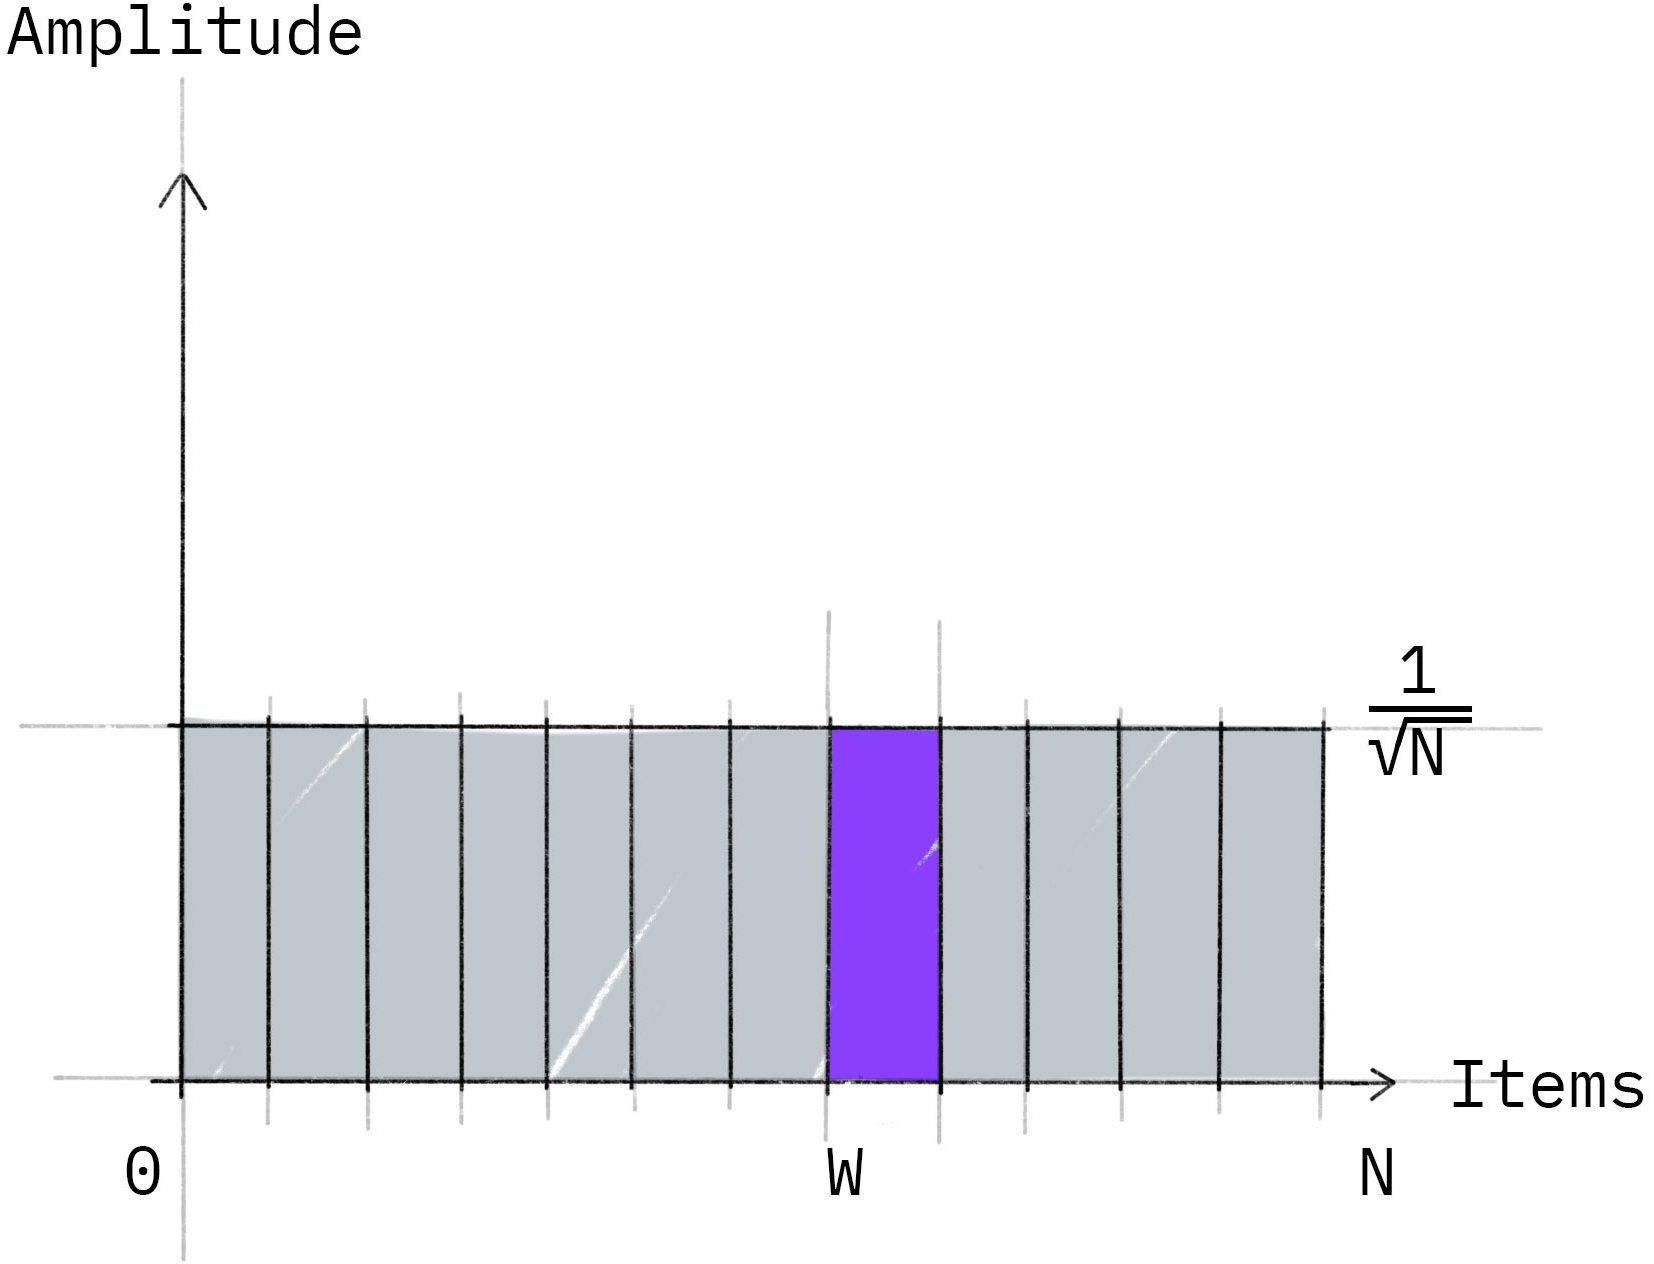
\includegraphics[width=0.5\linewidth]{content/assets/03_grovers_algorithm/grover_uniform.jpg}
    \caption{Grover starts out with the uniform distribution}
    \label{fig:grover_uniform}
\end{figure}

Then, it uses the verifier algorithm in a process to manipulate their probabilities until the correct entities' probabilities are very high, while the incorrect entities' probabilities are very low. This process is called amplitude amplification.

\begin{figure}[H]
    \centering
    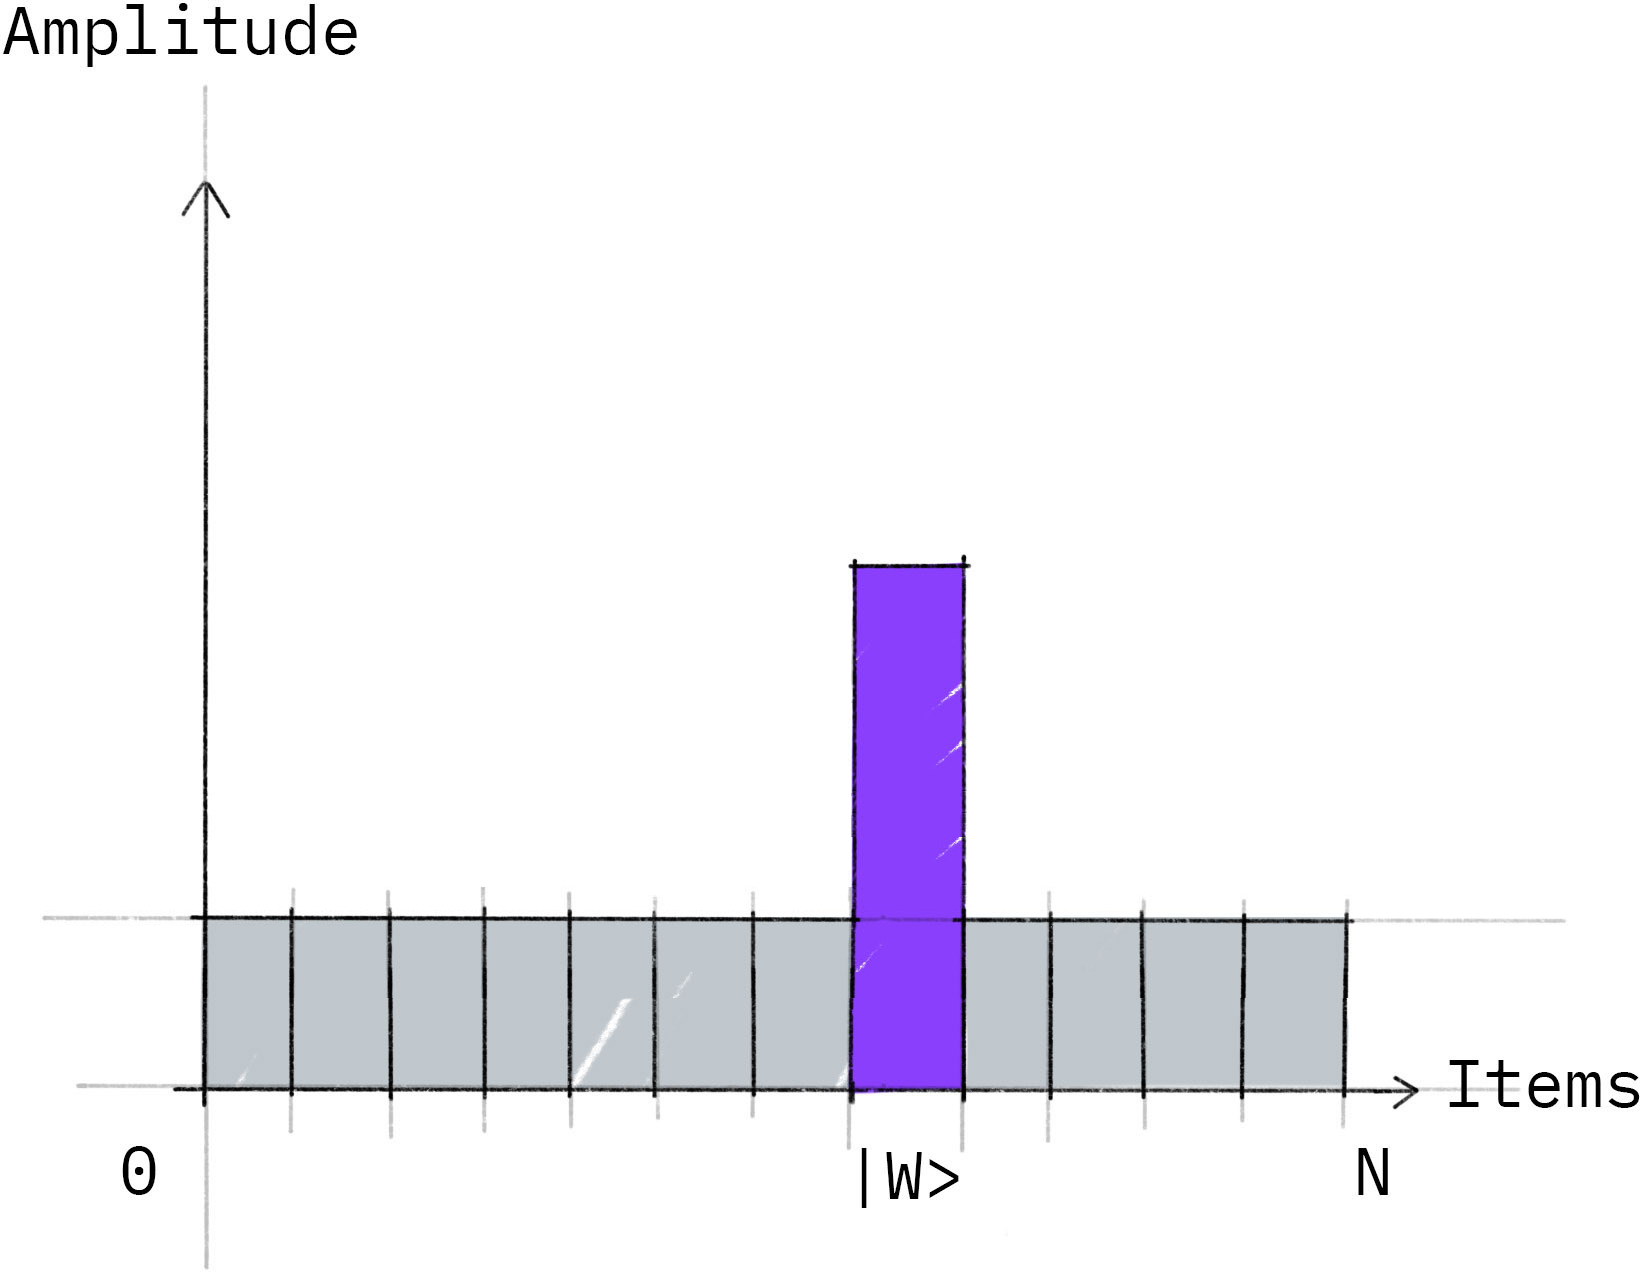
\includegraphics[width=0.5\linewidth]{content/assets/03_grovers_algorithm/grover_final.jpg}
    \caption{Grover amplifies the amplitude(s) of the correct solution(s)}
    \label{fig:grover_uniform}
\end{figure}

Finally, it samples from this probability distribution, which results in a correct solution entity with a high chance.

Working with a probability distribution over an exponentially large set of entities is only possible in a memory-efficient way on a quantum computer, thanks to the quantum physical nature of qubits.

A register of classical bits can only represent a single entity (encoded as a binary number), we would need separate registers to represent a set and we can only operate on the entire set in a linear fashion, one register at a time. In contrast, a register of quantum bits, or 'qubits' itself can represent a set of entities (a set of binary numbers) from the domain using the quantum physical phenomenon of superposition with a probability distribution over these elements.

The manipulation of these probabilities happens using quantum operators or gates, which are the basis of all quantum algorithms on gated general-purpose quantum computers.

However, we do not have access to this probability distribution or the high probability elements in it. The only thing we can do is read the register, which is an operation that samples a single entity from the current probability distribution in the register, destroying it in the process. We are unable to 'iterate' the contents of the register or know what the probability of the resulting element was from the sampling.

This is the reason why quantum parallelism is not as trivial as the name suggests: while we can run the computation itself in parallel, gaining access to the information that we stored in the register is difficult and destructive. Amplitude amplification is a technique that we use to fix this problem, however it requires $O(\sqrt{N})$ time, where $N$ is the size of the problem's domain, where $N=2^n$ if the quantum register has $n$ qubits.

One of the most important property of quantum registers is that they can even represent probability distributions, even ones where the individual qubits are \textbf{not independent}. This is called quantum entanglement.

One of the simplest forms of quantum entanglement are Bell states, which can occur between two qubits. In one of these Bell states, the probability distribution of our 2 qubit quantum registers is "$00$" with $50\%$ probability and "$11$" with $50\%$. Reading the contents of just the first qubit will result in a $50\%$ chance of reading a $0$ and a $50\%$ chance of reading a $1$. However, once we know the result from the first qubit, we can be $100\%$ sure, that when we sample the second qubit, we will get the same number as a result from it.




\chapter{Program felépítése}

\section{Regiszerek működése}

\section{Operátorok működése}

\chapter{Megoldandó feladat: Grover és Sudoku}

\section{Grover}

\section{Sudoku}

\chapter{Tesztelés}
\section{Memóriafelhasználás python kódban}
\section{Memóriafelhasználás C++ kódomban}

% \chapter{Introduction}

\section{Why are quantum computers interesting?}

Originally the idea of a quantum computer was suggested by Richard Feynman in a 1982 article (https://link.springer.com/article/10.1007/BF02650179), where he explains that currently existing classical computers are ill-equipped to deal with the complexity of the calculations required to simulate quantum physics. His suggestion was to replace the current hardware standard with one, which works based on quantum physical phenomena, thus giving it the capability to simulate the very thing it is based on.

The current computational model we use for classical computers is called the Turing-machine. These new types of computers are so different from classical ones that they run based on a completely different set of rules. Following the work of many computer scientists (Benioff, Deutsch, Bernstein and Vazirani), the computational model for Quantum computers was mathematically defined in the late 1980s: the Quantum Turing machine.

In the classical world, on the Turing machine, mathematicians and computer scientists have been struggling with the same problem for more than a hundred years: a solution to a set of computational problems that could unlock many real-world use cases in many industries [TODO: list examples]. These are called the NP-complete. This problem has eluded computer scientists for a century. This problem is so big that it is one of the famous Millennium Prize Problems set by the Clay Mathematics Institute, the P versus NP problem.

Using quantum parallelism quantum machines are able to operate on a large number of possible solutions at the same time. [TODO Scott Aaronson article about what we can do with Quantum computers]. This gives us hope that we could use Quantum Computers to solve the problems fast we are currently struggling in the classical world with.

\section{What is the motivation for this report?}

An interesting area for algorithmic research is bioinformatics. Many problems here have significant impact on our everyday lives since discoveries in this area can help us solve many of today’s major global problems, for example, aiding the creation of more effective medical treatments, advancing our understanding of genetic diseases, developing resistant crops to tackle a global food crisis or inventing novel technologies to reduce and revert environmental pollution. I am particularly interested in computer-aided drug design, where problems such as protein folding and molecular docking turn out to be NP-hard ones, which means that despite decades of effort, we have yet to come up with efficient solutions to them using classical computers.

In the past year I have been researching protein folding and how to implement it on a general-purpose quantum computer. I have ran into a significant problem: I was unable to run any experiments of usable size, mainly due to limitations in memory. Due to quantum parallelism, the memory requirements of running a quantum calculation simulation are super-exponential. In particular, there is one component in Qiskit, which seemed to come back in any form of model I have tried to implement: a quantum gate for taking the sum of $n$ qubits, called the WeightedAdder class. 

[TODO: Kép a weighted adder class kapujáról qiskitből]

This component came up, because a natural way to encode protein structures is by creating a 3D grid and laying the aminoacid chain down on it:

[TODO: Valami kép, ezt nem kéne magyarázni sokat.]

From a single vertex in a 3D grid, we can step in $6$ directions: up, down, left, right, inwards and outwards. We can encode these naturally, using one-hot encoding, by introducing $6$ bits of information.

[TODO: kép a directionökről]

If we assume that the chain starts in the origin, then we can encode a chain shape by giving the directions of the $(n-1)$ steps it takes.

[TODO: kép...]

A chain like this is viable, when it doesn't cross over itself. A chain's optimality is assessed by counting how many pairs of various aminoacids are neighbouring each other. To answer both of these questions, we must be able to calculate relative distances between any two points of the chain. Using the directinal one-hot encoding model, these questions can be answered by taking the sum of some qubits.

Using these operations, we can create a quantum oracle, that assesses the optimality of a particular chain and use Grover's quantum search algorithm to find the best possible solution.

Unfortunately, while Qiskit itself is open-source, it's architecture (similarly to other quantum computing frameworks) is designed from the core to store the matrices of various operations (such as the WeightedAdder operation) in its memory and retrieve this information during simulation. This means that I am unable to correct this single operation in Qiskit.

\section{What is the scope of this report?}

In order to reduce the memory requirements for any quantum computation simulation, we have to be able to reduce storing large operation matrices in memory whenever we can. This requires a completely different architecture.

The scope of this report is designing and implementing this architecture, particularly solving the problem with WeightedAdder. While the original motivation for the focus on this specific component comes from protein folding, bioinformatics is out of scope for this paper. Instead, I will be taking a much simpler problem, a generic version of Sudoku, which also requires the WeightedAdder component and Grover-search to be solved.

% \chapter{Quantum computing}

Algorithms in quantum computing are derived from the postulates of quantum mechanics. These fundamental rules define how a quantum computer operates, and therefore they are essential for any discourse on quantum algorithms.

\section{The postulates of quantum mechanics}

This introduction is based on the following books: Quantum Computing and Communications by Sándor Imre and Ferenc Balázs~\cite{ImreSandor}, Quantum Computing by Mika Hirvensalo~\cite{Hirvensalo} and Quantum Walks and Search Algorithms by Renato Portugal~\cite{Portugal}.

\lineparagraph{Postulate I. State space}

The state of an isolated physical system can be described using a unit length \textit{state vector} in a Hilbert space (i.e. complex linear vector space), or \textit{state space}, equipped with an inner product.

\begin{definition}[Qubit]
A state vector in the 2 dimensional Hilbert space ($H_2$) is a qubit. The base vectors in this space are
\end{definition}

\begin{align*}
\ket{0} = \begin{pmatrix} 1 \\ 0 \end{pmatrix} \text{, and } \ket{1} = \begin{pmatrix} 0 \\ 1 \end{pmatrix}.
\end{align*}

A generic qubit is written in the form

\begin{align*}
a\ket{0} + b\ket{1} = \begin{pmatrix} a \\ b \end{pmatrix}
\end{align*}

where $a, b \in{} \mathds{C}$ and $|a|^2 + |b|^2 = 1$.

\begin{definition}[Superposition]

A quantum system is said to be in \textit{superpotion}, if its state vector is a linear combination of multiple basis states.

For example $a\ket{0} + b\ket{1}$ is in a superposition of the basis states $\ket{0}$ and $\ket{1}$, with probability amplitudes $a$ and $b$.

\end{definition}

\lineparagraph{Postulate II. Evolution}
\label{PostulateII}

The time evolution of an isolated physical system is described using unitary transformation, which depends only on the starting and finishing time of the evolution.

A \textit{quantum algorithm} is a sequence of unitary operators applied to an initial state.

\begin{definition}[Unitary matrix]
\label{Unitary}

$\mathbf{U}$ is unitary if $\mathbf{U}^{\dagger} = \mathbf{U}^{-1}$  \cite{HalmosLinearAlgebra}.

The following definitions are equivalent:

\begin{enumerate}
    \item $\mathbf{U}$'s rows form an orthonormal basis of $\mathds{C}^n$.
    \item $\mathbf{U}$'s columns form an orthonormal basis of $\mathds{C}^n$.
    \item $\mathbf{U}$ is an isometry: it is injective and preserves length.
    \item $\mathbf{U}$ preserves the inner product.
\end{enumerate}

\end{definition}

\lineparagraph{Postulate III. Measurement}

A quantum measurement is defined by a set of measurement operators $\{\mathbf{M}_m\}$, where $m$ stands for the possible results of the measurement. The probability of measuring $m$ if the system is in state $\ket{v}$ is

\begin{align*}
    P(m | \ket{v}) = \bra{v} \mathbf{M}_m^{\dagger} \mathbf{M}_m \ket{v}.
\end{align*}

The state of the system after measuring $m$ is then

\begin{align*}
    \ket{v'} = \frac{\mathbf{M}_m\ket{v}}{\sqrt{\bra{v} \mathbf{M}_m^{\dagger} \mathbf{M}_m \ket{v}}}.
\end{align*}

The set of measurement operators have to satisfy the following \textit{completeness relation}:

\begin{align*}
    \sum\limits_{m}  \mathbf{M}_m^{\dagger} \mathbf{M}_m = I,
\end{align*}

due to

\begin{align*}
    1 = \sum\limits_{m} P(m | \ket{v}) = \sum\limits_{m} \bra{v} \mathbf{M}_m^{\dagger} \mathbf{M}_m \ket{v}.
\end{align*}

\linesubparagraph{Projective measurement}\label{PostulateIIIProjective}

To distinguish a set of orthonormal states $\{\ket{\varphi_m}\}$, the corresponding measurement operators can be produced as $\mathbf{P}_m = \ket{\varphi_m}\bra{\varphi_m}$, with the following properties.

\begin{property}[$\mathbf{P}_m$ is self adjoint]

\begin{align*}
\mathbf{P}_m^{\dagger} = \mathbf{P}_m
\end{align*}

Since

\begin{align*}
\mathbf{P}_m^{\dagger} =
(\ket{\varphi_m}\bra{\varphi_m})^{\dagger} =
\bra{\varphi_m}^{\dagger}\ket{\varphi_m}^{\dagger} =
\ket{\varphi_m}\bra{\varphi_m} =
\mathbf{P}_m.
\end{align*}

\end{property}

\begin{property}[$\mathbf{P}_m$ is a projection]

\begin{align*}
\mathbf{P}_m\mathbf{P}_m = \mathbf{P}_m
\end{align*}

Since
\begin{align*}
\mathbf{P}_m\mathbf{P}_m =
(\ket{\varphi_m}\bra{\varphi_m})(\ket{\varphi_m}\bra{\varphi_m}) =
\ket{\varphi_m}(\bra{\varphi_m}\ket{\varphi_m})\bra{\varphi_m} =
\ket{\varphi_m}1\bra{\varphi_m} =
\ket{\varphi_m}\bra{\varphi_m} =
\mathbf{P}_m.
\end{align*}

\end{property}

\begin{property}[The $\mathbf{P}_m$ are orthogonal]

\begin{align*}
m \neq n \Rightarrow \mathbf{P}_m\mathbf{P}_n = \mathbf{0}
\end{align*}

Since
\begin{align*}
\mathbf{P}_m\mathbf{P}_n =
(\ket{\varphi_m}\bra{\varphi_m})(\ket{\varphi_n}\bra{\varphi_n}) =
\ket{\varphi_m}(\bra{\varphi_m}\ket{\varphi_n})\bra{\varphi_n} =
\ket{\varphi_m}0\bra{\varphi_n} =
\mathbf{0}.
\end{align*}

\end{property}

From these properties follows, that the probability of measuring $m$ in case of a projective measurement is

\begin{align*}
P(m | \ket{v}) =
\bra{v}\mathbf{P}_m^{\dagger}\mathbf{P}_m \ket{v} =
\bra{v}\mathbf{P}_m\mathbf{P}_m\ket{v} = 
\bra{v}\mathbf{P}_m\ket{v} =
\bra{v}\ket{\varphi_m}\bra{\varphi_m}\ket{v} = |\bra{\varphi_m}\ket{v}|^2.
\end{align*}

For example, the value of a qubit can be any unit length vector in $H_2$, however when we measure it, we will receive one of the base vectors of $H_2$. For $a\ket{0} + b\ket{1}$ we measure $0$ with probability $|a|^2$ and $1$ with probability $|b|^2$.

\lineparagraph{Postulate IV. Composite systems}
\label{PostulateIV}

The state space of an isolated composite physical system is the \textit{tensor product} of the state spaces of the individual components. The current state vector of the composite system is the \textit{tensor product} of the current state vectors of the individual systems.

If $V_1,\dots,V_n$ are the state spaces of the individual systems, then $V_1 \otimes \dots \otimes V_n$ is the composite state space and for $\ket{v_1} \in V_1, \dots, \ket{v_n} \in V_n$ state vectors, $\ket{v_1} \otimes \dots \otimes \ket{v_n} = \ket{v_1,\dots,v_n}$ is the state vector of the composite system.

\begin{definition}[Tensor product]

The tensor product $\mathbf{A} \otimes \mathbf{B}$ of matrix $\mathbf{A}_{(r \times s)}$ and matrix $\mathbf{B}_{(t \times u)}$ is of size $(rt \times su)$ and is defined as follows \cite{HalmosLinearAlgebra}:

\begin{align*}
\text{For }
\mathbf{A} = \begin{pmatrix}
    a_{11} & a_{12} & \dots  & a_{1s} \\
    a_{21} & a_{22} & \dots  & a_{2s} \\
    \vdots & \vdots & \ddots & \vdots \\
    a_{r1} & a_{r2} & \ddots & a_{rs}
\end{pmatrix}
\text{, and }
\mathbf{B} = \begin{pmatrix}
    b_{11} & b_{12} & \dots  & b_{1u} \\
    b_{21} & b_{22} & \dots  & b_{2u} \\
    \vdots & \vdots & \ddots & \vdots \\
    b_{t1} & b_{t2} & \ddots & b_{tu}
\end{pmatrix}
\end{align*}

\begin{align*}
\mathbf{A} \otimes \mathbf{B} = \begin{pmatrix}
    a_{11}\mathbf{B} & a_{12}\mathbf{B} & \dots  & a_{1s}\mathbf{B} \\
    a_{21}\mathbf{B} & a_{22}\mathbf{B} & \dots  & a_{2s}\mathbf{B} \\
    \vdots  & \vdots  & \ddots & \vdots  \\
    a_{r1}\mathbf{B} & a_{r2}\mathbf{B} & \ddots & a_{rs}\mathbf{B}
\end{pmatrix}
\end{align*}

\end{definition}

and has the following properties:

\begin{property}[Associativity]
\begin{align*}
  (\mathbf{A} \otimes \mathbf{B}) \otimes \mathbf{C} = \mathbf{A} \otimes (\mathbf{B} \otimes \mathbf{C})
\end{align*}
\end{property}

\begin{property}[Mixed product property]
\label{TensorMixedProduct}

If the corresponding matrices are compatible, then

\begin{align*}
  (\mathbf{A} \otimes \mathbf{B})(\mathbf{C} \otimes \mathbf{D}) = (\mathbf{A}\mathbf{C}) \otimes (\mathbf{B}\mathbf{D}),
\end{align*}
\end{property}

and as an immediate consequence, we obtain 

\begin{align*}
  (\mathbf{A} \otimes \mathbf{I})(\mathbf{I} \otimes \mathbf{B}) = \mathbf{A} \otimes \mathbf{B}.
\end{align*}

\begin{definition}[Quantum register]

The composite system of $n$ qubits is a \textit{quantum register}, having the composite state space

\begin{align*}
H_2^{\otimes{}n} = H_2 \otimes H_2 \otimes ... \otimes H_2
\end{align*}

and for $\ket{q_{n-1}} \in H_2, \dots, \ket{q_{0}} \in H_2$ individual state vectors, the composite state vector is

\begin{align*}
\ket{q_{n-1}} \otimes \dots \otimes \ket{q_{0}} = \ket{q_{n-1},\dots,q_0}.
\end{align*}

\end{definition}

\begin{definition}[Entangled state]
Any state consisting of multiple qubits, that is not decomposable, i.e. that can not be written in the form of a composite system of qubits is \textit{entangled}.
\end{definition}

For example, the state $\frac{1}{\sqrt{2}}(\ket{00} + \ket{11})$ is entangled, since it can not be written in the form

\begin{align*}
(a_0\ket{0} + a_1\ket{1})\otimes(b_0\ket{0}+b_1\ket{1}) = a_0b_0\ket{00}+a_0b_1\ket{01}+a_1b_0\ket{10}+a_1b_1\ket{11}
\end{align*}

since that would require from $a_0b_0 = a_1b_1 = \frac{1}{\sqrt{2}}$, for all coefficients to be non-zero and from $a_0b_1 = a_1b_0 = 0$ for either $a_0$ or $b_1$ and either $a_1$ or $b_0$ to be zero, which is a contradiction.
% \chapter{Simulator software}

In this chapter, I present the simulator software I wrote. I discuss the currently available solutions, why I chose to write the software, the architecture, the components and design patterns I used, the challenges I faced during the development and the solutions I found.

\section{Currently available solutions}

Since publicly accessible quantum computers currently only have around 5-10 qubits, it is not viable at the moment to run quantum walks on a real quantum computer. Hence why, when I started researching quantum walks, I quickly began looking into simulator software. While there are many of these currently available, most of them have at least one of the following issues:

\begin{enumerate}
\item Not maintained and developed anymore: the last commit was years ago.
\item Written in a low-level language, like C++, in a script-like fashion, with a prominent focus on memory and performance optimization while neglecting readability, modularity and extensibility.
\item Works exclusively on a specific type of graph, for example, $n$-dimensional lattices only.
\item Unable to compare and contrast classical and quantum walks on the same graph, running only quantum simulations.
\item Hard to understand as a novice.
\end{enumerate}

There is no general, open-source solution available that is designed and developed using sound software engineering practices and an architecture that allows for experimentation with different kinds of graphs with both classical and quantum simulations available.

I intend my solution to be valuable for research purposes while also providing a readable open-source codebase for college students to study the algorithm.

\section{Architecture}

The architecture of my simulator program employs the Strategy design pattern, which is described in the following way:

''Define a family of algorithms, encapsulate each one, and make them interchangeable. Strategy lets the algorithm vary independently from clients that use it.''~\cite{DesignPatterns}

% \begin{figure}[H]
%  \includegraphics[width=\linewidth]{./figures/program/strategy.png}
%  \caption{UML diagram for the Strategy design pattern from~\cite{DesignPatterns}}
% \end{figure}

This is a great design pattern for research purposes since it facilitates experimentation with various algorithms for the same purpose. It also makes the code easily readable, as the Strategy interface provides an abstraction layer between the Context and the concrete implementation.

\section{Language choice}

With the specified goals and the architecture in mind, I needed a language that is object-oriented, easily readable by beginners and has extensive capabilities for using complex numbers, linear algebra and plotting. For these purposes, I choose the Python language. Python is concise, it reads like pseudocode and has libraries such as NumPy, SciPy and Matplotlib, and so on, covering all areas of data science. Furthermore, it is well-known and extensively used by researchers with no software engineering background, allowing for easier collaboration.

\section{High level design}

The source code of the software can be divided into three parts:

\begin{itemize}
    \item Graph models
    \item Simulators
    \item Running, configuration and result collection
\end{itemize}

% \begin{figure}[H]
%  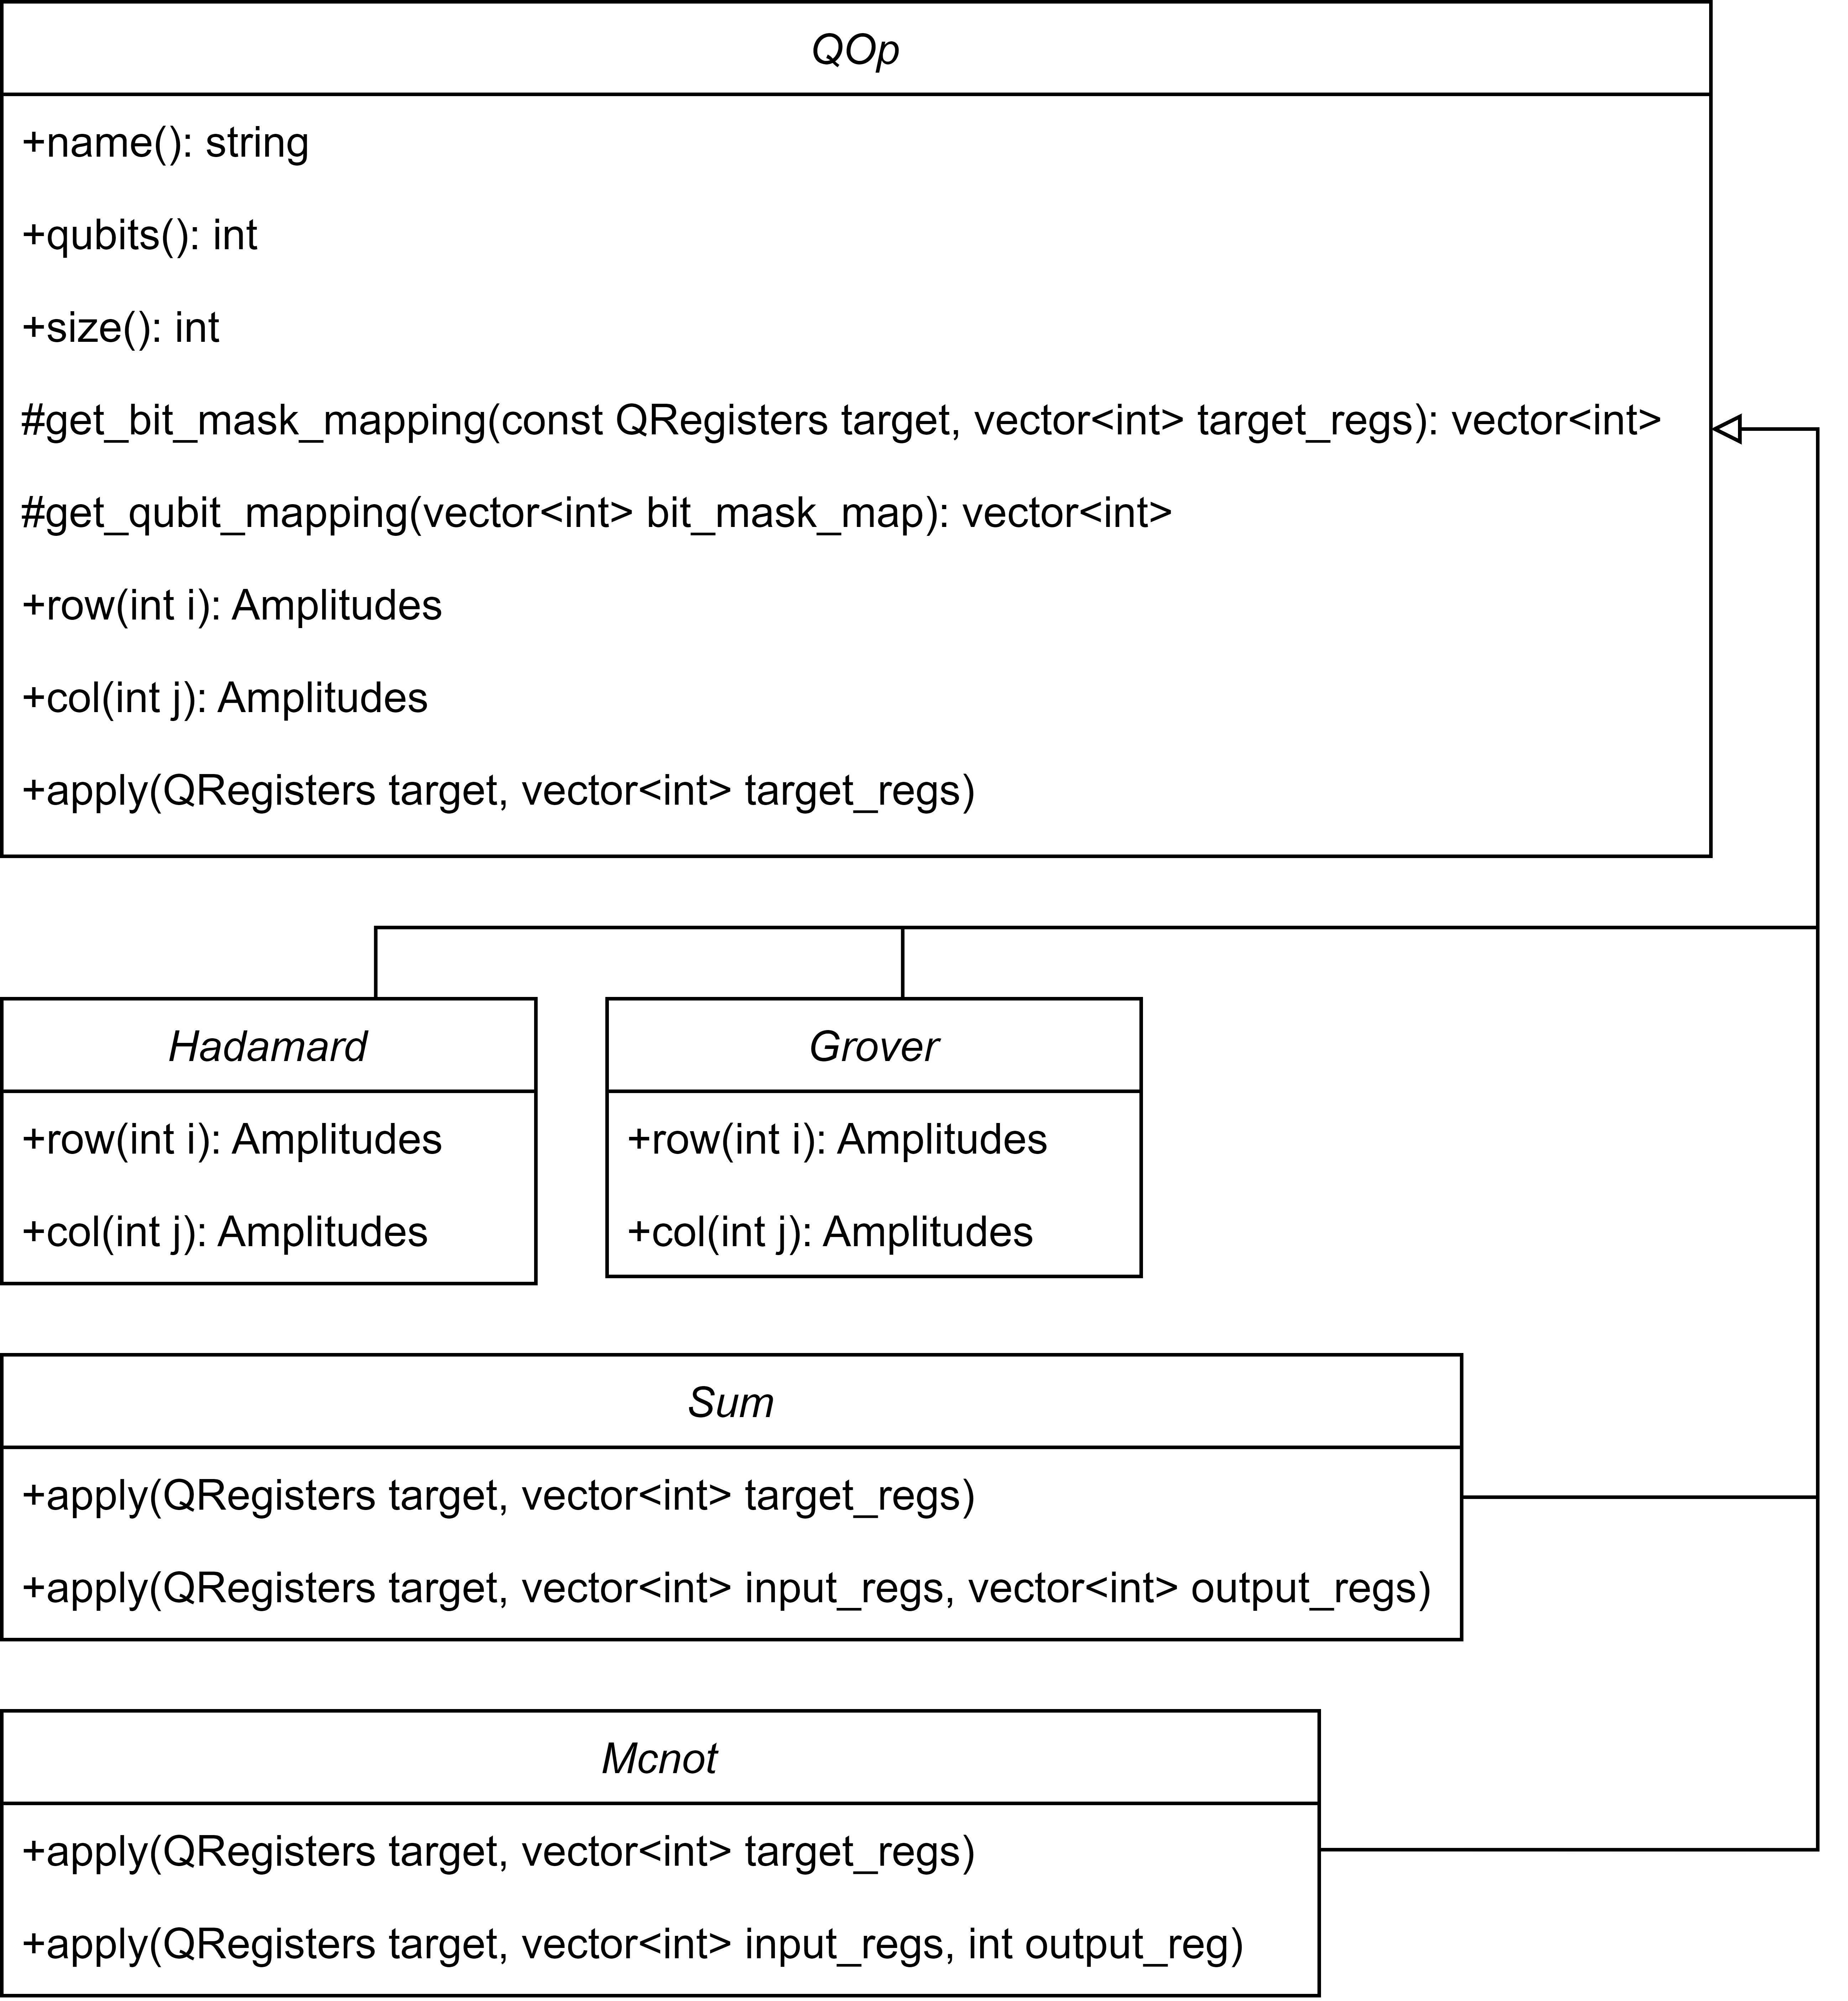
\includegraphics[width=\linewidth]{./figures/program/uml.png}
%  \caption{UML diagram for the Graph models and Simulators}
%\end{figure}

On the UML diagram above, the SubGraph class is a Strategy, with the following ConcreteStrategy implementations:

\begin{itemize}
    \item BinaryTree
    \item Bipartite
    \item Circle
    \item Grid
    \item Hypercube
    \item Path
    \item Random
\end{itemize}

Each of these employs an oracle that calculates neighbouring vertices on-the-fly.

Furthermore, the Simulator is also a Strategy, implemented by the Classical and the Quantum classes, the latter using the Coin Strategy, implemented by the Hadamard, Grover and Fourier (DFT) classes.

(For a cleaner diagram, I did not picture the SubGraph and Coin implementations.)

\subsection{Graph models}

I ran several experiments on various graphs while researching quantum graph walks, including paths, circles, bipartite graphs, hypercubes, and grids. Initially, I directly generated and stored their adjacency matrices, however, I quickly ran into memory scaling issues with this approach. Furthermore, in quantum research, graphs are typically built like 'Legos', glueing together a few common types, which was challenging to do with my original approach.

To combat these issues, I switched from the adjacency matrix representation to the oracle representation. The oracle is a function that returns the neighbours of a given vertex. Since I was using common graphs, I could calculate neighbouring indexes on-the-fly without storing anything about these graphs and only querying what is needed at the current step, dramatically reducing the memory requirements of the graph models.

\subsection{Simulators}

I implemented a classical and a quantum simulator class. The quantum simulator can currently simulate directed $k$ regular graphs, however since the permutation matrix decomposition, or in the undirected case, the edge coloring of the matrix is an NP-complete problem, in the current setup, the graph oracle must be implemented in a way that returns the neighbours in the same color order for all inputs. Since the human programmer designs the oracle, this is not a critical limitation at the moment. I have implemented a check as a safety guard to ensure the resulting shift matrices are unitary in case an error is made while coding one of the oracles.

\subsection{Running, configuration and result collection}

Using the above classes, I developed a framework in which experimental runs can be configured very quickly. The results of the run are collected in an aggregated Latex document, using Matplotlib for creating various graphics. It contains the given graph, the named type of the subgraphs, the adjacency matrices, the distribution results of the simulations, including empirical hitting and mixing times and the eigenvalues and eigenvectors of the evolution operators. In the following chapter, I present several examples collected from these Latex reports of my experiments.

\subsection{Availability}

My simulator software is available under the open-source MIT license on my personal Github account, under the following link:

\url{https://github.com/nemkin/qmem}


% TODO \chapter{Acknowledgement}

% List of Figures, Tables
%\listoffigures\addcontentsline{toc}{chapter}{\listfigurename}
%\listoftables\addcontentsline{toc}{chapter}{\listtablename}

% Bibliography
\nocite{*}
\addcontentsline{toc}{chapter}{\bibname}
\bibliography{include/mybib}

% Appendices
\include{content/end/appendices}

\end{document}
